
%%%%%%%%%%%%%%%%%%%%%%%%%%%%%%%%%%%%%%%%%%%%%%%%%%%%%%%%%%%%%%%%%%%%%%%
%%%%%%%%%%%%%%%%%%%%%%%%%%%%%%%%%%%%%%%%%%%%%%%%%%%%%%%%%%%%%%%%%%%%%%% 
%%%%%%%%%%%       								 Preamble				         	                                                        %%%%%%%%%% 
%%%%%%%%%%%%%%%%%%%%%%%%%%%%%%%%%%%%%%%%%%%%%%%%%%%%%%%%%%%%%%%%%%%%%%% 
%%%%%%%%%%%%%%%%%%%%%%%%%%%%%%%%%%%%%%%%%%%%%%%%%%%%%%%%%%%%%%%%%%%%%%% 
\documentclass[10pt]{beamer}
\usepackage{setspace}
\usepackage{color}
\usepackage{amsmath,lmodern}
\usepackage{hyperref}
\usepackage{graphicx}
\usepackage{multirow}
\usepackage{tikz}
\usetikzlibrary{fit,shapes.misc}
\usepackage{pdflscape}
\usepackage{amsmath}
\usepackage{lscape}
\usepackage{multirow}
\usepackage{enumerate}
\usepackage{epstopdf}
\usepackage{pdfpages}
\usepackage{appendixnumberbeamer}
\usepackage{color,soul}
\usepackage{grffile}
\usepackage{float}
\usepackage{relsize}
\usepackage{tcolorbox}
\newcounter{nodemarkers}
\usepackage{tikz}
\newcommand{\toplinesmall}{%
  \tikz[remember picture,overlay] {%
    \draw[blue,thick] ([yshift=-1cm, xshift=.9cm]current page.north west)
             -- ([yshift=-1cm,xshift=3.6cm]current page.north west);}}
             
\newcommand{\toplinemedium}{%
  \tikz[remember picture,overlay] {%
    \draw[blue,thick] ([yshift=-1cm, xshift=.9cm]current page.north west)
             -- ([yshift=-1cm,xshift=6.2cm]current page.north west);}}
 
 \newcommand{\toplinelarge}{%
  \tikz[remember picture,overlay] {%
    \draw[blue,thick] ([yshift=-1cm, xshift=.9cm]current page.north west)
             -- ([yshift=-1cm,xshift=8.9cm]current page.north west);}}           
             
 \newcommand{\toplinexlarge}{%
  \tikz[remember picture,overlay] {%
    \draw[blue,thick] ([yshift=-1cm, xshift=.9cm]current page.north west)
             -- ([yshift=-1cm,xshift=12cm]current page.north west);}}                       
             
\setbeamertemplate{footline}
{
  \leavevmode%
  \hbox{%
  \begin{beamercolorbox}[wd=.333333\paperwidth,ht=2.25ex,dp=1ex,center]{author in head/foot}%
    \usebeamerfont{author in head/foot}{\textcolor{blue}{ECON311}}
  \end{beamercolorbox}%
  \begin{beamercolorbox}[wd=.333333\paperwidth,ht=2.25ex,dp=1ex,center]{title in head/foot}%
    \usebeamerfont{title in head/foot}{\textcolor{blue}{Winter 2026}}
  \end{beamercolorbox}%
  \begin{beamercolorbox}[wd=.333333\paperwidth,ht=2.25ex,dp=1ex,right]{date in head/foot}%
    \usebeamerfont{date in head/foot}{\textcolor{blue}{Lecture 4 \: \: \: \: \: \: \: }
    \insertframenumber{} / \inserttotalframenumber\hspace*{2ex}} 
  \end{beamercolorbox}}%
  \vskip0pt%
}
\newtheorem{proposition}[theorem]{Proposition}

\newcommand\marktopleft[1]{%
    \tikz[overlay,remember picture] 
        \node (marker-#1-a) at (-0.2,1.2ex) {};%
}
\newcommand\markbottomright[1]{%
    \tikz[overlay,remember picture] 
        \node (marker-#1-b) at (0.16,-1ex) {};%
    \tikz[overlay,remember picture,thick,inner sep=4pt]
        \node[draw,rectangle,rounded corners, blue, fit=(marker-#1-a.center) (marker-#1-b.center)] {};%
}

\setbeamertemplate{caption}{\raggedright\insertcaption\par}
\setbeamertemplate{itemize items}[ball]
\setbeamertemplate{itemize subitem}[triangle]
\setbeamertemplate{itemize subsubitem}[triangle]
\tcbset{colframe=white,colback=white,nobeforeafter}
\beamertemplatenavigationsymbolsempty
\addtobeamertemplate{frametitle}{\vspace*{0.19cm}}{\vspace*{0cm}}


%%%%%%%%%%%%%%%%%%%%%%%%%%%%%%%%%%%%%%%%%%%%%%%%%%%%%%%%%%%%%%%%%%%%%%%
%%%%%%%%%%%%%%%%%%%%%%%%%%%%%%%%%%%%%%%%%%%%%%%%%%%%%%%%%%%%%%%%%%%%%%% 
%%%%%%%%%  									    Define Title									                                       %%%%%%%%%
%%%%%%%%%%%%%%%%%%%%%%%%%%%%%%%%%%%%%%%%%%%%%%%%%%%%%%%%%%%%%%%%%%%%%%%
%%%%%%%%%%%%%%%%%%%%%%%%%%%%%%%%%%%%%%%%%%%%%%%%%%%%%%%%%%%%%%%%%%%%%%% 
\title{ECON 311} 
\author{Lecture 4: Economic Growth}
\date{}
\AtBeginSection[]
{
 \begin{frame}<beamer>
 \tableofcontents[currentsection]
 \end{frame}
}
%%%%%%%%%%%%%%%%%%%%%%%%%%%%%%%%%%%%%%%%%%%%%%%%%%%%%%%%%%%%%%%%%%%%%%%
%%%%%%%%%%%%%%%%%%%%%%%%%%%%%%%%%%%%%%%%%%%%%%%%%%%%%%%%%%%%%%%%%%%%%%% 
%%%%%%%% 						     				Document								                                                %%%%%%%%
%%%%%%%%%%%%%%%%%%%%%%%%%%%%%%%%%%%%%%%%%%%%%%%%%%%%%%%%%%%%%%%%%%%%%%%
%%%%%%%%%%%%%%%%%%%%%%%%%%%%%%%%%%%%%%%%%%%%%%%%%%%%%%%%%%%%%%%%%%%%%%% 
\begin{document}
\setbeamercovered{transparent}

\begin{frame}
\maketitle
\end{frame}

%%%%%%%%%%%%%%%%%%%%%%%%%%%%%%%%%%%%%%%%%%%%%%%%%%%%%%%%%%%%%%%%%%%%%%%
%%%%%%%%%%%%%%%%%%%%%%%%%%%%%%%%%%%%%%%%%%%%%%%%%%%%%%%%%%%%%%%%%%%%%%% 
%%%%%%%% 						     				Introduction	             		                                		  %%%%%%%%
%%%%%%%%%%%%%%%%%%%%%%%%%%%%%%%%%%%%%%%%%%%%%%%%%%%%%%%%%%%%%%%%%%%%%%%
%%%%%%%%%%%%%%%%%%%%%%%%%%%%%%%%%%%%%%%%%%%%%%%%%%%%%%%%%%%%%%%%%%%%%%% 


\section{Introduction to Long-Run Growth}

\begin{frame}
\frametitle{\: \: \: Introduction to Growth}
\toplinelarge
\begin{itemize}
\item Standards of living in industrialized countries have greatly increased over the past few centuries.
\begin{itemize}
\vspace{.11in}
\item E.g. Averages incomes today in North America and Western Europe are between 50 and 300 times larger than two centuries ago.
\end{itemize}
\vspace{.11in}
\item This increase in standards of living has been a very recent phenomena in human history.
\begin{itemize}
\vspace{.11in}
\item For most of their history (before the Industrial Revolution), humans lived barely above subsistence levels.
\end{itemize}
\vspace{.11in}
\item Economic growth has been very uneven across time.
\begin{itemize}
\vspace{.11in}
\item E.g. the productivity growth slowdown of 1990's
\end{itemize}
\vspace{.11in}
\item Economic growth has been very uneven across countries. 
\begin{itemize}
\vspace{.11in}
\item E.g. growth miracles (Japan, South Korea, Singapore), growth disasters (Argentina, Sub-Saharan countries)
\end{itemize}
\end{itemize}
\end{frame}

\begin{frame}
\frametitle{\: \: \: Economic Growth Over the Very Long Run}
\toplinexlarge
\begin{figure}
\centering
\includegraphics[scale=.63]{econ_growth.png}
\caption{Source: Macroeconomics, Jones}
\end{figure}
\end{frame}

\begin{frame}
\frametitle{\: \: \: Economic Growth Over Time}
\toplinelarge
\begin{figure}
\centering
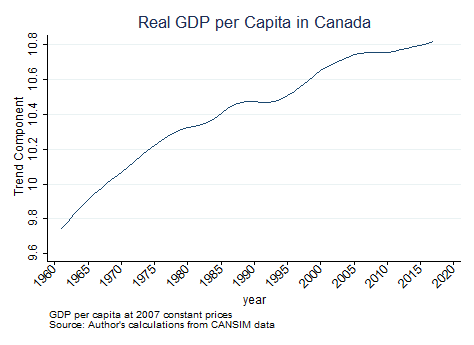
\includegraphics[scale=.56]{RGDP_trend}
\end{figure}
\end{frame}

\begin{frame}
\frametitle{\: \: \: Defining Economic Growth}
\toplinelarge
\begin{itemize}
\item Let $g$ be a constant growth rate over a period of time, then ...
\begin{eqnarray*}
y_{t+T}=y_{t}(1+g)^{T} 
\end{eqnarray*}
\item Important properties of growth rates:
\begin{enumerate}
\vspace{.11in}
\item (Rule of 70) Let $y_{t+T}=2y_t$ and , then
\begin{eqnarray*}
T \approx \frac{0.7}{g}
\end{eqnarray*}
\item In general, the time it takes for a series to increase by a certain ratio does not depend on the initial level.
\vspace{.11in}
\item Algebraic properties of growth rates (let the variable $i$ grow at a constant growth rate $g_i$):
\begin{eqnarray*}
\begin{array}{cl} 
z=\frac{x}{y} & \Rightarrow g_z = g_x-g_y \\
z=x \cdot y &\Rightarrow g_z = g_x+g_y \\
z=x^a \text{ (where $a$ is a constant)} & \Rightarrow g_z = a\cdot g_x
\end{array}
\end{eqnarray*}
\end{enumerate}
\end{itemize}
\end{frame}

\begin{frame}
\frametitle{\: \: \: GDP per capita trend revisited}
\toplinelarge
\begin{columns}
\begin{column}{0.5\linewidth}
\begin{itemize}
\item We can calculate average growth rates over a period of time $T$ as follows:
\begin{eqnarray*}
\overline{g}=\left(\frac{y_{t+T}}{y_t}\right)^{\frac{1}{T}}-1
\end{eqnarray*}
\item To separate the trend from the cycle, we choose a particular period of time and change the annual GDP per capita by that rate
\end{itemize}
\end{column}
\begin{column}{0.5\linewidth}
\begin{figure}
\centering
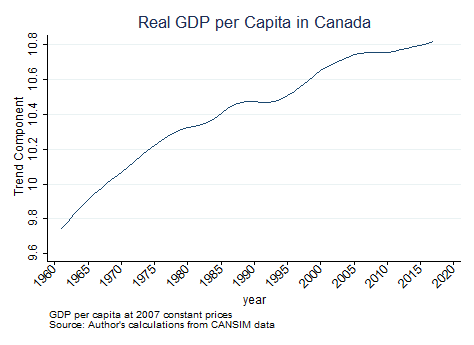
\includegraphics[scale=.34]{RGDP_trend}
\end{figure}
\end{column}
\end{columns}
\end{frame}

\begin{frame}
\frametitle{\: \: \: Graphing Growth Rates}
\toplinelarge
\begin{figure}
\centering
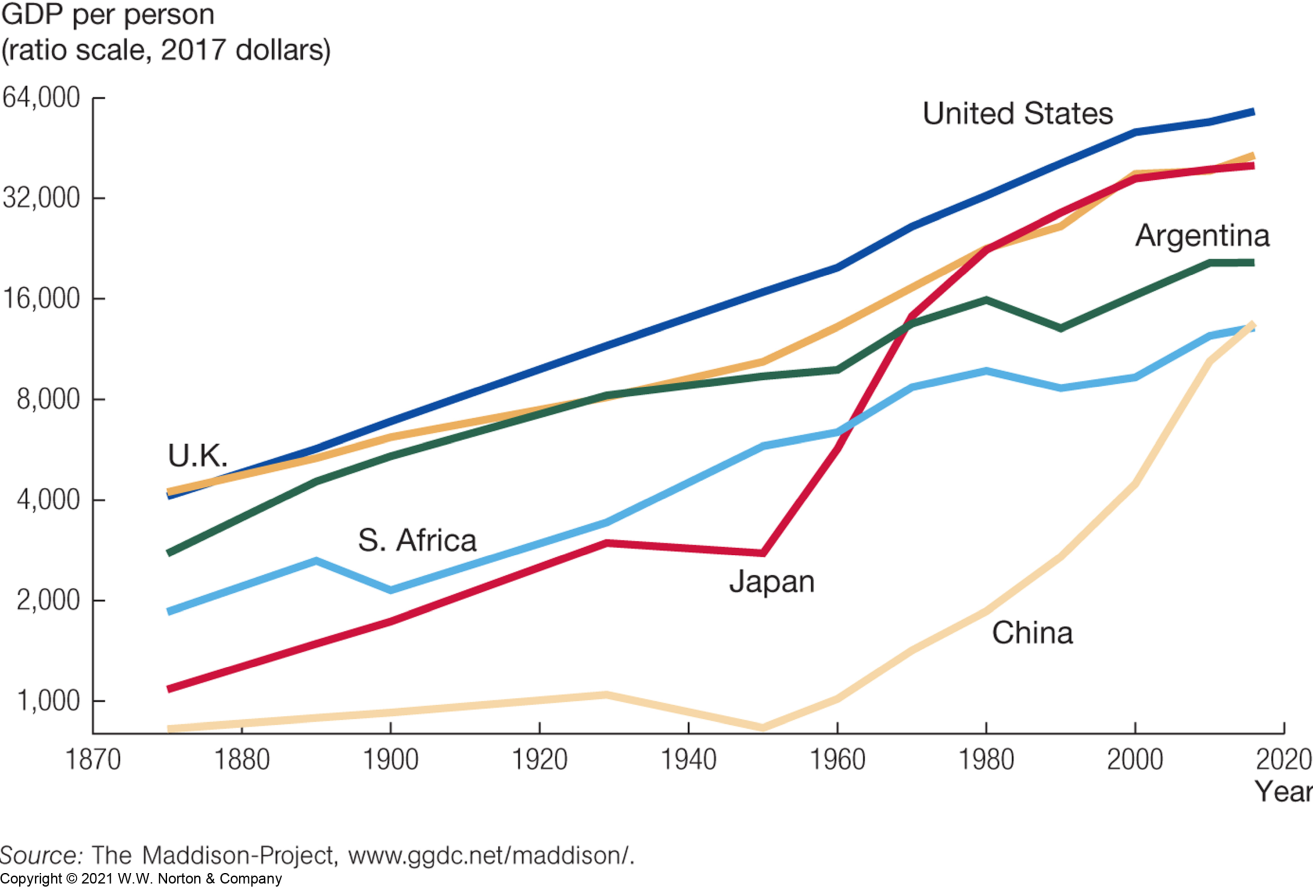
\includegraphics[scale=.35]{GDP_country_world}
\caption{Source: Macroeconomics, Jones}
\end{figure}
\end{frame}

\begin{frame}
\frametitle{\: \: \: The power of economic growth}
\toplinelarge
\begin{figure}
\centering
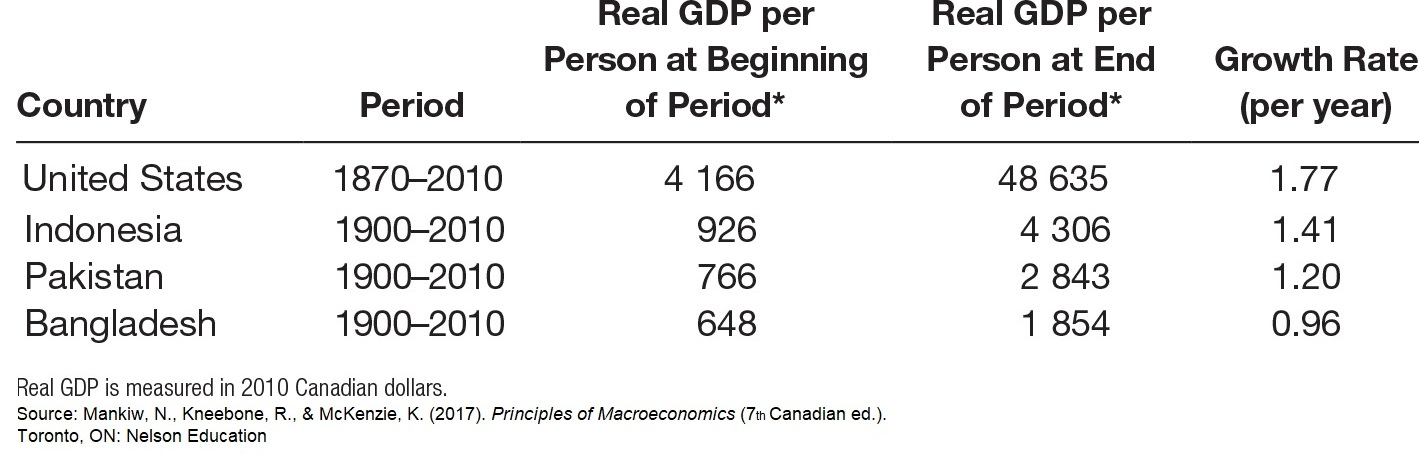
\includegraphics[scale=.8]{power_of_growth}
\end{figure}
\begin{itemize}
\only<1>{
\item At average growth rates it will take Bangladesh around 340 years, Pakistan around 237 years and Indonesia around 172 years to reach levels of real GDP per capita similar to US in 2010.}
\only<2>{
\item If average growth were to increase be a \textit{quarter} of a percent, it would take Bangladesh around 270 years (diff. of 70 years), Pakistan around 196 years (diff. of 41 years) and Indonesia around 146 years (diff. of 26 years) to reach levels of real GDP per capita similar to US in 2010.} 
\end{itemize}
\end{frame}

\begin{frame}
\frametitle{\: \: \: Growth Rates Among Developed Countries}
\toplinexlarge
\begin{figure}
\centering
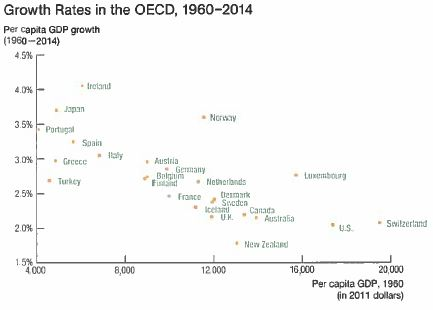
\includegraphics[scale=.75]{convergence}
\caption{Source: Advanced Macroeconomics, D. Romer}
\end{figure}
\end{frame}

\begin{frame}
\frametitle{\: \: \: Long-Run Growth}
\toplinemedium
\begin{itemize}
\item Given the importance of long-run growth for well-being, we will study the classical model of economic growth.
\vspace{.11in}
\item The goal is to learn the mechanics of the model and its insights concerning the dynamics of long-run growth across time and countries.
\vspace{.11in}
\item The ultimate objective of research on economic growth is to study possible economic policies for raising growth in poor countries to bring GDP per capita closer to the level of rich countries.
\begin{itemize}
\vspace{.11in}
\item To that end, we will confront this model with the data to see if it offers meaningful answers to our central objective.
\end{itemize}
\end{itemize}
\end{frame}   


\section{A Production Model}

\begin{frame}
\frametitle{\: \: \: Introduction}
\toplinemedium
\begin{itemize}
\item To understand the causes of the great differences in production across time and countries, we first write down the following  production function:
\begin{eqnarray*}
Y=F(K,L)=\overline{A}K^{\alpha}L^{(1-\alpha)} &, & \alpha \leq 1
\end{eqnarray*}  
\item This production function has several theoretical properties that facilitates the analysis of empirical implications of differences in $K$ and $L$.
\end{itemize}
\end{frame}

\begin{frame}
\frametitle{\: \: \: Properties of the Production Function}
\toplinexlarge
The Cobb-Douglas Production Function has the following properties:
\vspace{.15in}
\only<1>{
\begin{enumerate}
\item Diminishing returns to $K$ and $L$:
\end{enumerate}
\begin{columns}
\begin{column}{0.5\linewidth}
\begin{eqnarray*}
\begin{array}{l}
MPK=\frac{\partial Y}{\partial K}=\alpha \overline{A} \left( \frac{L}{K} \right)^{(1-\alpha)} \\[1.4ex]
MPL=\frac{\partial Y}{\partial L }=(1-\alpha) \overline{A} \left( \frac{K}{L} \right)^{\alpha}
\end{array}
\end{eqnarray*}
\end{column}
\begin{column}{0.5\linewidth}
\begin{figure}
\centering
\caption{Diminishing Returns to $i$ for $i=K,L$}
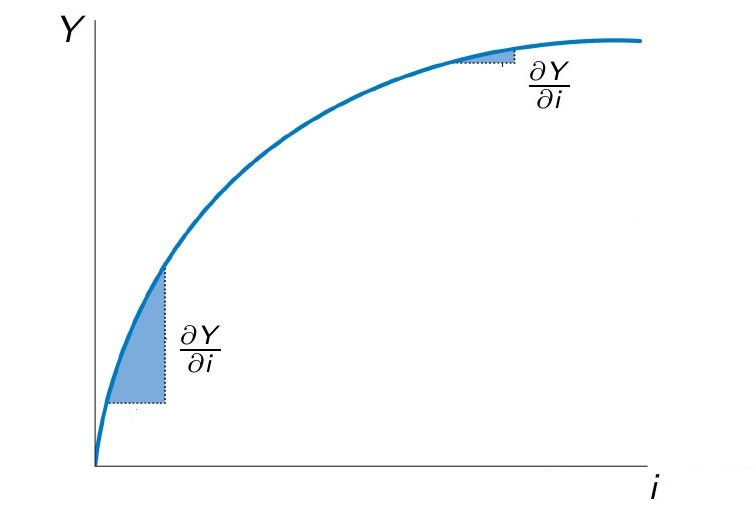
\includegraphics[scale=.28]{diminishing_returns}
\end{figure}
\end{column}
\end{columns}
\begin{itemize}
\item Differences in $K$ accumulation per person has different implications at different levels of development
\end{itemize}}
\only<2>{
\begin{enumerate}
\setcounter{enumi}{1}
\item Constant Returns to Scale:
\end{enumerate}
\begin{columns}
\begin{column}{0.5\linewidth}
\begin{eqnarray*}
\begin{array}{l}
F(\lambda K, \lambda L)=\lambda F(K,L) \\[1.4ex]
F(\lambda K, \lambda L)=\lambda \underbrace{\overline{A}K^{\alpha}L^{(1-\alpha)}}_{F(K,L)}
\end{array}
\end{eqnarray*}
\end{column}
\begin{column}{0.5\linewidth}
\begin{figure}
\centering
\caption{Constant Returns to scale}
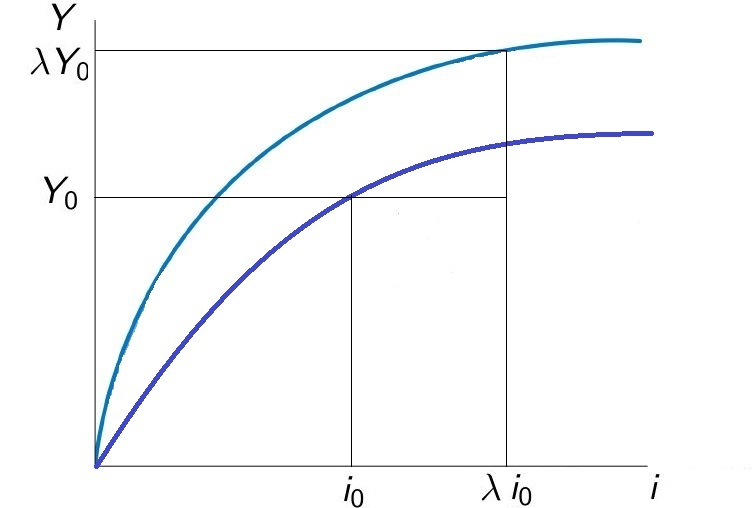
\includegraphics[scale=.28]{constant_returns_scale}
\end{figure}
\end{column}
\end{columns}
\begin{itemize}
\item Population size matters for total income but does not for income per capita
\end{itemize}}
\end{frame}

\begin{frame}
\frametitle{\: \: \: Solving for Production Parameters}
\toplinexlarge
\begin{itemize}
\item To take this model to the data, we need ...
\begin{itemize}
\vspace{.11in}
\item to assign value to the parameter, $\alpha$ 
\vspace{.11in}
\item and study how differences in the exogenous variables, $K$, $L$, $\overline{A}$, result in differences in endogenous variable, $Y$.
\end{itemize}
\vspace{.11in}
\item It turns out that from the optimal decision of firms to rent $K$ and hire $L$, we obtain:
\begin{eqnarray*}
\begin{array}{lcl} 
\frac{wL^*}{Y^*}=(1-\alpha) &, & \frac{rK^*}{Y^*}=\alpha
\end{array}
\end{eqnarray*}
\vspace{.11in}
\item We can obtain this from the income approach to measuring GDP: $\alpha=\frac{1}{3}$
\end{itemize}
\end{frame} 

\begin{frame}
\frametitle{\: \: \: Development Accounting}
\toplinelarge
\begin{itemize}
\item Our main concerned is to measure GDP per capita differences, so we expressed the production in per capita terms:
\begin{eqnarray*}
\begin{array}{lll}
y=\overline{A}k^{\frac{1}{3}} &, y=\frac{Y}{L}, &k=\frac{K}{L}
\end{array}
\end{eqnarray*}
\item We are going to assume that a country uses all of its resources to produce:
\begin{eqnarray*}
\begin{array}{lll}
k=\overline{k}&, &\overline{k}=\frac{\overline{K}}{\overline{L}}
\end{array}
\end{eqnarray*}
\item We observe differences in $\overline{k}$ but, because we do not observe differences in $\overline{A}$,...
\begin{itemize}  
\vspace{.11in}
\item we will assume that it is the same for all countries.
\end{itemize}
\vspace{.11in}
\item In the following exercise, we will calculate the output of country $c$ relative to the $US$:
\begin{eqnarray*}
\frac{y_c}{y_{US}}=\left(\frac{\overline{k}_{c}}{\overline{k}_{US}}\right)^{\frac{1}{3}}
\end{eqnarray*}
\end{itemize}  
\end{frame}

\begin{frame}
\frametitle{\: \: \: Development Accounting}
\toplinelarge
\begin{figure}
\centering
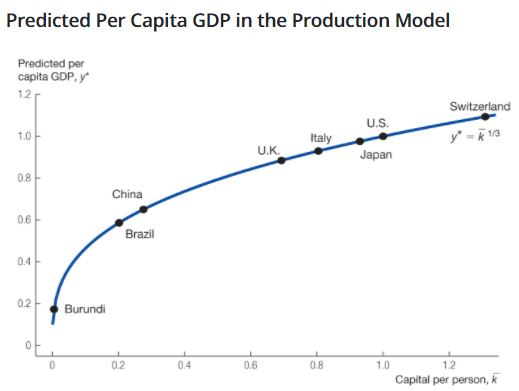
\includegraphics[scale=.65]{figure_44}
\end{figure}
\end{frame}

\begin{frame}
\frametitle{\: \: \: Development Accounting}
\toplinelarge
\begin{figure}
\centering
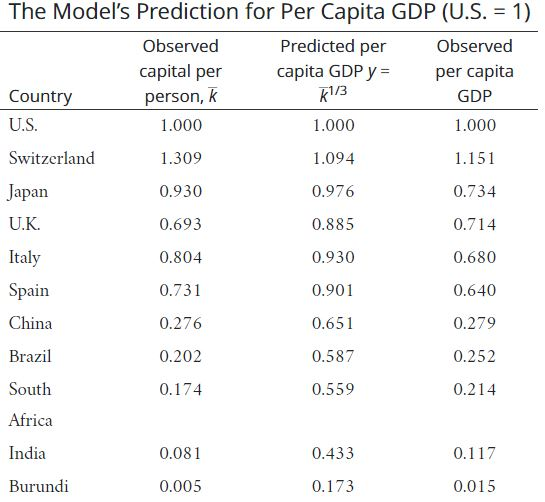
\includegraphics[scale=.48]{table_43}
\end{figure}
\end{frame}



\begin{frame}
\frametitle{\: \: \: Development Accounting}
\toplinelarge
\begin{figure}
\centering
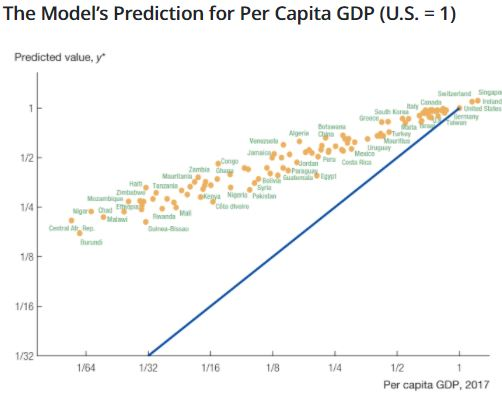
\includegraphics[scale=.65]{figure_45}
\end{figure}
\end{frame}

\begin{frame}
\frametitle{\: \: \:  Model with only $k$ and constant $\overline{A}$ }
\toplinexlarge
\begin{itemize}
\item The model without $\overline{A}$ differences underestimate differences in output per capita.
\vspace{.11in}
\item On average, $y$ in industrialized countries is 10 times larger than in non-industrialized countries:
\begin{eqnarray*}
10=\frac{\overline{A}^{ind}\left(k^{ind}\right)^{\frac{1}{3}}}{\overline{A}^{nind}\left(k^{nind}\right)^{\frac{1}{3}}} 
\end{eqnarray*}
\begin{itemize}
\item If we assume that $\overline{A}^{ind}=\overline{A}^{nind}$, then ...
\begin{eqnarray*}
10^3=1000=\frac{k^{ind}}{k^{nind}}
\end{eqnarray*}
\begin{itemize}
\item There is no empirical evidence of such large differences.
\end{itemize}
\end{itemize}
\vspace{.11in}
\item Presumably,  differences in $\overline{A}$ play a big role in accounting for differences in $y$.
\begin{itemize}
\vspace{.11in}
\item We cannot be certain of this because differences in $\overline{A}$ are unobserved in general.
\end{itemize}
\end{itemize}
\end{frame}










\end{document}


